\documentclass[aspectratio=169]{../latex_main/tntbeamer}  % you can pass all options of the beamer class, e.g., 'handout' or 'aspectratio=43'
\usepackage{dsfont}
\usepackage{bm}
\usepackage[english]{babel}
\usepackage[T1]{fontenc}
%\usepackage[utf8]{inputenc}
\usepackage{graphicx}
\graphicspath{ {./figures/} }
\usepackage{algorithm}
\usepackage[ruled,vlined,algo2e,linesnumbered]{algorithm2e}
\usepackage{hyperref}
\usepackage{booktabs}
\usepackage{mathtools}

\usepackage{amsmath,amssymb}

\DeclareMathOperator*{\argmax}{arg\,max}
\DeclareMathOperator*{\argmin}{arg\,min}

\usepackage{amsbsy}
\newcommand{\vect}[1]{\bm{#1}}
%\newcommand{\vect}[1]{\boldsymbol{#1}}

\usepackage{pgfplots}
\pgfplotsset{compat=1.16}
\usepackage{tikz}
\usetikzlibrary{trees} 
\usetikzlibrary{shapes.geometric}
\usetikzlibrary{positioning,shapes,shadows,arrows,calc,mindmap}
\usetikzlibrary{positioning,fadings,through}
\usetikzlibrary{decorations.pathreplacing}
\usetikzlibrary{intersections}
\pgfdeclarelayer{background}
\pgfdeclarelayer{foreground}
\pgfsetlayers{background,main,foreground}
\tikzstyle{activity}=[rectangle, draw=black, rounded corners, text centered, text width=8em]
\tikzstyle{data}=[rectangle, draw=black, text centered, text width=8em]
\tikzstyle{myarrow}=[->, thick, draw=black]

% Define the layers to draw the diagram
\pgfdeclarelayer{background}
\pgfdeclarelayer{foreground}
\pgfsetlayers{background,main,foreground}

% Requires XeLaTeX or LuaLaTeX
%\usepackage{unicode-math}

\usepackage{fontspec}
%\setsansfont{Arial}
\setsansfont{RotisSansSerifStd}[ 
Path=../latex_main/fonts/,
Extension = .otf,
UprightFont = *-Regular,  % or *-Light
BoldFont = *-ExtraBold,  % or *-Bold
ItalicFont = *-Italic
]
\setmonofont{Cascadia Mono}[
Scale=0.8
]

% scale factor adapted; mathrm font added (Benjamin Spitschan @TNT, 2021-06-01)
%\setmathfont[Scale=1.05]{Libertinus Math}
%\setmathrm[Scale=1.05]{Libertinus Math}

% other available math fonts are (not exhaustive)
% Latin Modern Math
% XITS Math
% Libertinus Math
% Asana Math
% Fira Math
% TeX Gyre Pagella Math
% TeX Gyre Bonum Math
% TeX Gyre Schola Math
% TeX Gyre Termes Math

% Literature References
\newcommand{\lit}[2]{\href{#2}{\footnotesize\color{black!60}[#1]}}

%%% Beamer Customization
%----------------------------------------------------------------------
% (Don't) Show sections in frame header. Options: 'sections', 'sections light', empty
\setbeamertemplate{headline}{empty}

% Add header logo for normal frames
\setheaderimage{
	% 
\includegraphics[height=\logoheight]{figures/TNT_darkv4.pdf}
	
\includegraphics[height=\logoheight]{../latex_main/figures/luh_logo_rgb_0_80_155.pdf}
	% 
\includegraphics[height=\logoheight]{figures/logo_tntluh.pdf}
}

% Header logo for title page
\settitleheaderimage{
	% 
\includegraphics[height=\logoheight]{figures/TNT_darkv4.pdf}
	
\includegraphics[height=\logoheight]{../latex_main/figures/luh_logo_rgb_0_80_155.pdf}
	% 
\includegraphics[height=\logoheight]{figures/logo_tntluh.pdf}
}

% Title page: tntdefault 
\setbeamertemplate{title page}[tntdefault]  % or luhstyle
% Add optional title image here
%\addtitlepageimagedefault{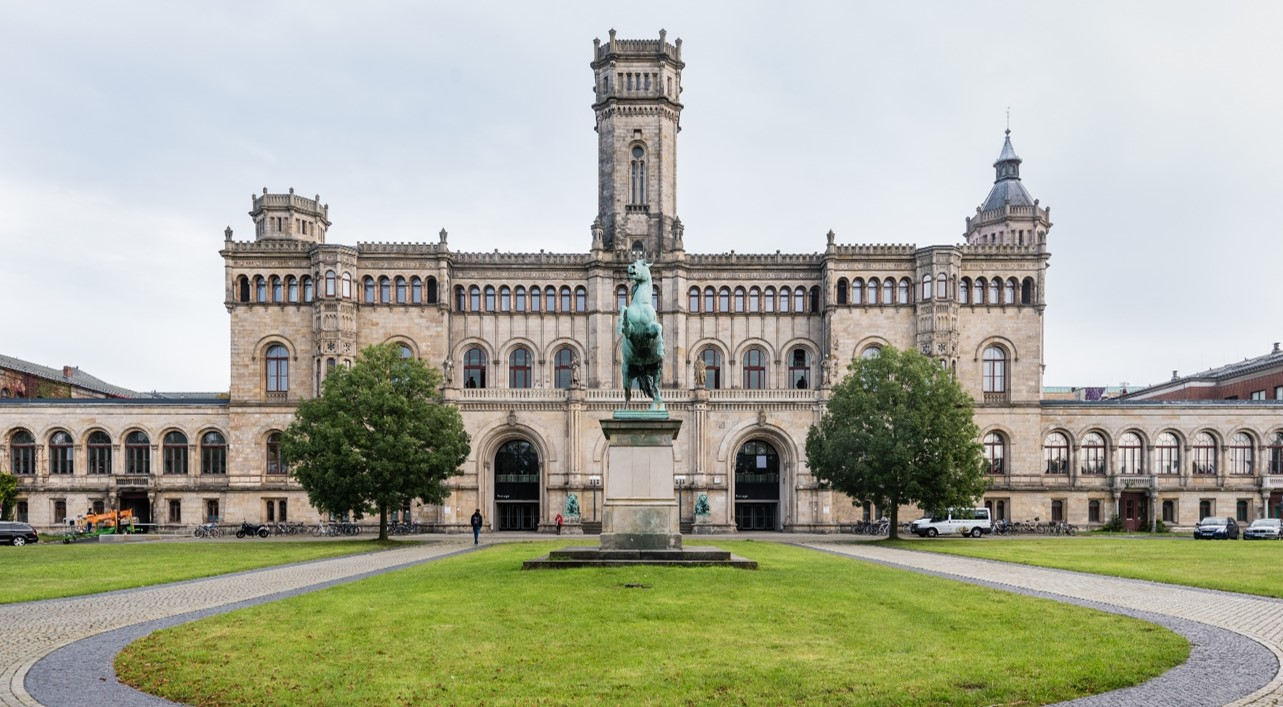
\includegraphics[width=0.65\textwidth]{figures/luh_default_presentation_title_image.jpg}}

% Title page: luhstyle
% \setbeamertemplate{title page}[luhstyle]
% % Add optional title image here
% \addtitlepageimage{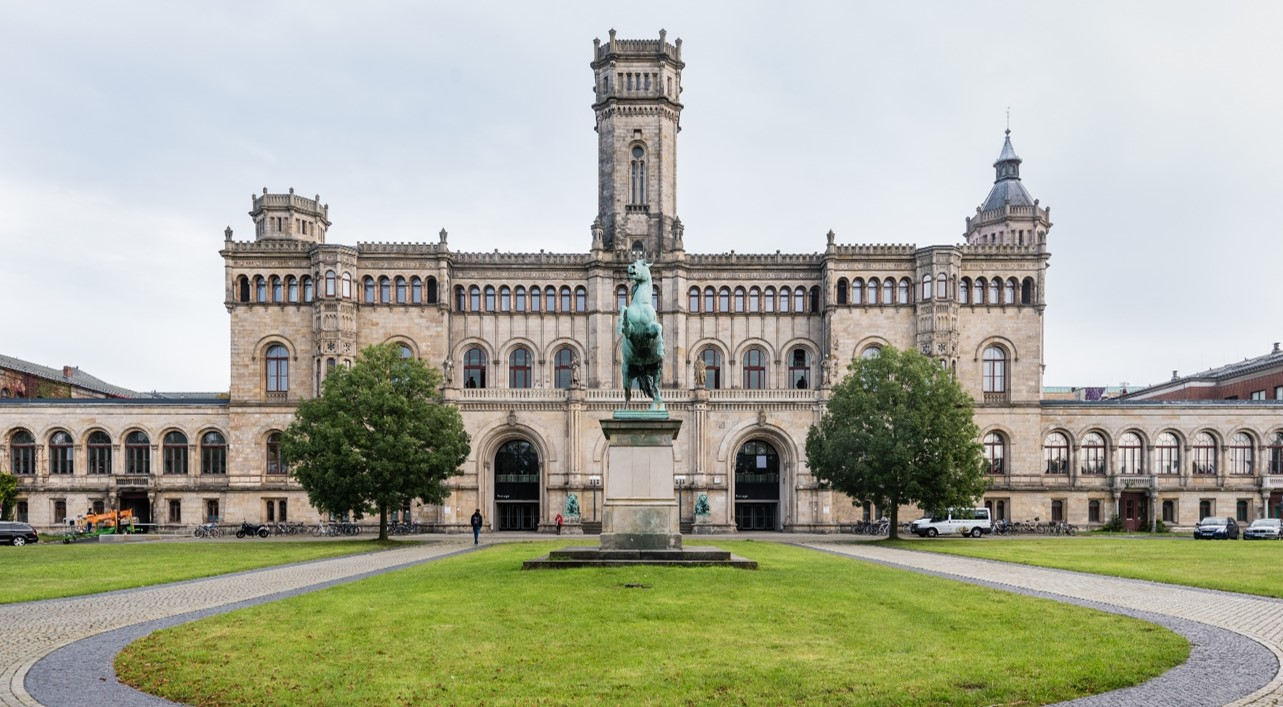
\includegraphics[width=0.75\textwidth]{figures/luh_default_presentation_title_image.jpg}}

\author[Abedjan \& Lindauer]{Ziawasch Abedjan \& Marius Lindauer\\[1em]
	
\includegraphics[height=\logoheight]{../latex_main/figures/luh_logo_rgb_0_80_155.pdf}\qquad
	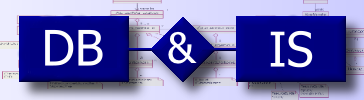
\includegraphics[height=\logoheight]{../latex_main/figures/DBIS_Kurzlogo.png}\qquad

\includegraphics[height=\logoheight]{../latex_main/figures/TNT_darkv4}\qquad

\includegraphics[height=\logoheight]{../latex_main/figures/L3S.jpg}	}
\date{Summer Term 2022; \hspace{0.5em} {
\includegraphics[height=1.5em]{../latex_main/figures/Cc-by-nc-sa_icon.svg.png}}; based on \href{https://ds100.org/fa21/}{[DS100]}
}


%%% Custom Packages
%----------------------------------------------------------------------
% Create dummy content
\usepackage{blindtext}

% Adds a frame with the current page layout. Just call \layout inside of a frame.
\usepackage{layout}


%%% Macros
%\renewcommand{\vec}[1]{\mathbf{#1}}
% \usepackage{bm}
%\let\vecb\bm

\title[Introduction]{DS: Data Cleaning and EDA}
\subtitle{Granularity, Scope, and Temporality}

\graphicspath{ {./figure/} }
%\institute{}


\begin{document}
	
	\maketitle
	
	\begin{frame}{Key Data Properties to Consider in EDA}
	    \begin{itemize}
	        \item Structure -- the “shape” of a data file
	        \item \textbf{Granularity -- how fine/coarse is each datum}
	        \item Scope -- how (in)complete is the data
	        \item Temporality -- how is the data situated in time
	        \item Faithfulness -- how well does the data capture “reality”
	    \end{itemize}
	\end{frame}
	
	
	
	\begin{frame}{Granularity}
	    \centering
	    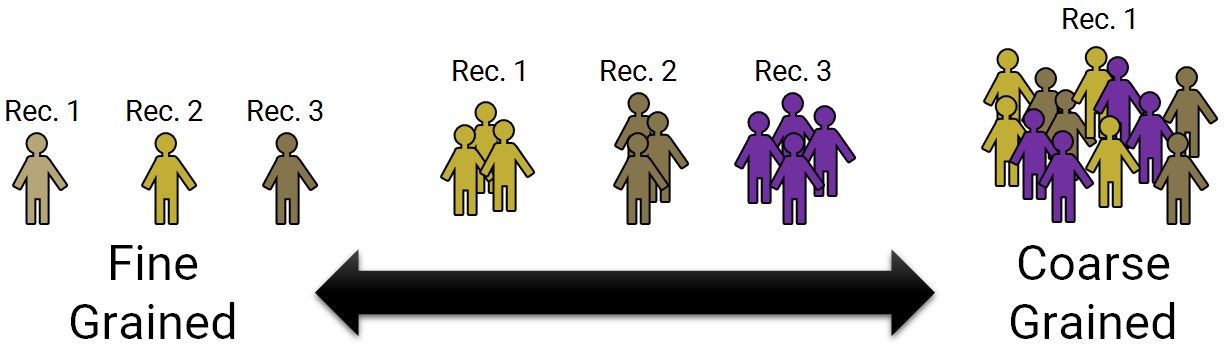
\includegraphics[scale=.35]{Bild18}
	    \begin{itemize}
	        \item What does each record represent?
	        \begin{itemize}
	            \item Examples: a purchase, a person, a group of users
	        \end{itemize}
	        \item Do all records capture granularity at the same level?
	        \begin{itemize}
	            \item Some data will include summaries (aka rollups) as records
	        \end{itemize}
	        \item If the data are coarse how was it aggregated?
	        \begin{itemize}
	            \item Sampling, averaging, …
	        \end{itemize}
	    \end{itemize}
	\end{frame}
	
	
	
	\begin{frame}{Key Data Properties to Consider in EDA}
	    \begin{itemize}
	        \item Structure -- the “shape” of a data file
	        \item Granularity -- how fine/coarse is each datum
	        \item \textbf{Scope -- how (in)complete is the data}
	        \item Temporality -- how is the data situated in time
	        \item Faithfulness -- how well does the data capture “reality”
	    \end{itemize}
	\end{frame}
	
	
	
	\begin{frame}{Scope}
	    \begin{itemize}
	        \item Does my data cover my area of interest?
	        \begin{itemize}
	            \item Example: I am interested in studying crime in California but I only have Berkeley crime data. 
	        \end{itemize}
	        \item Is my data too expansive?
	        \begin{itemize}
	            \item Example: I am interested in student grades for DS100 but have student grades for all statistics classes.
	            \item Solution: Filtering ⇒ Implications on sample?
	            \begin{itemize}
	                \item If the data is a sample I may have poor coverage after filtering …
	            \end{itemize}
	        \end{itemize}
	        \item Does my data cover the right time frame?
	        \begin{itemize}
	            \item More on this in temporality … 
	        \end{itemize}
	    \end{itemize}
	\end{frame}
	
	
	
	\begin{frame}{Revisiting the Sampling Frame}
	    \begin{itemize}
	        \item The sampling frame is the population from which the data was sampled.
	        \begin{itemize}
	            \item Note that this may not be the population of interest.
	        \end{itemize}
	        \item How complete/incomplete is the frame (and its data)? 
	        \item How is the frame/data situated in place?
	        \item How well does the frame/data capture reality?
	        \item How is the frame/data situated in time? 
	    \end{itemize}
	\end{frame}
	
	
	\begin{frame}{Key Data Properties to Consider in EDA}
	    \begin{itemize}
	        \item Structure -- the “shape” of a data file
	        \item Granularity -- how fine/coarse is each datum
	        \item Scope -- how (in)complete is the data
	        \item \textbf{Temporality -- how is the data situated in time}
	        \item Faithfulness -- how well does the data capture “reality”
	    \end{itemize}
	\end{frame}
	
	
	
	
	\begin{frame}{Temporality}
	    \begin{itemize}
	        \item Data changes – when was the data collected?
	        \item What is the meaning of the time and date fields?
	        \begin{itemize}
	            \item When the “event” happened?
	            \item When the data was collected or was entered into the system?
	            \item Date the data was copied into a database (look for many matching timestamps)
	        \end{itemize}
	        \item Time depends on where! (Time zones & daylight savings)
	        \begin{itemize}
	            \item Learn to use datetime python library
	            \item Multiple string representation (depends on region): 07/08/09?
	        \end{itemize}
	        \item Are there strange null values?
	        \begin{itemize}
	            \item January 1$^{st}$ 1970, January 1$^{st}$ 1900
	        \end{itemize}
	        \item Is there periodicity? Diurnal patterns
	    \end{itemize}
	\end{frame}
	
	
	
	
	\begin{frame}{Unix Time / POSIX Time}
	    \begin{columns}
	    \begin{column}{.7\textwidth}
	    
	  
	    
	    \begin{itemize}
	        \item Time measured in seconds since January 1$^{st}$ 1970
	        \begin{itemize}
	            \item Minus leap seconds …
	        \end{itemize}
	        \item Unix time follows Coordinated Universal Time (UTC)
	        \begin{itemize}
	            \item International time standard 
	            \item Measured at 0 degrees latitude
	            \begin{itemize}
	                \item Similar to Greenwich Mean Time (GMT)
	            \end{itemize}
	            \item No daylight savings 
	            \item Time codes 
	        \end{itemize}
	        \item Time Zones
	        \begin{itemize}
	            \item San Francisco (UTC-8) without daylight savings
	        \end{itemize}
	    \end{itemize}
	    \bigskip
	    \url{https://en.wikipedia.org/wiki/Coordinated_Universal_Time}
	      \end{column}
	      
	      
	      \begin{column}{.3\textwidth}
	              \begin{figure}
	                  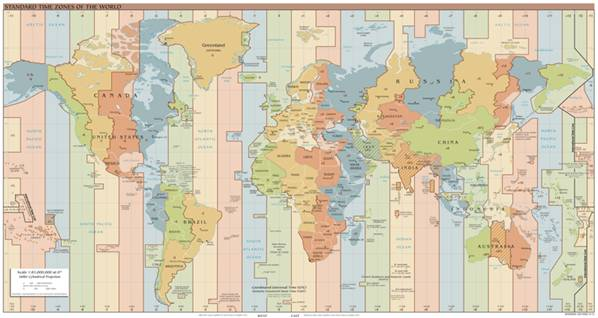
\includegraphics[scale=.45]{Bild19}
	              \end{figure}
	      \end{column}
	    \end{columns}
	\end{frame}
\end{document}